\section{Performance}

\subsection{Module testing}

\begin{figure}[hbt] 
\centering 
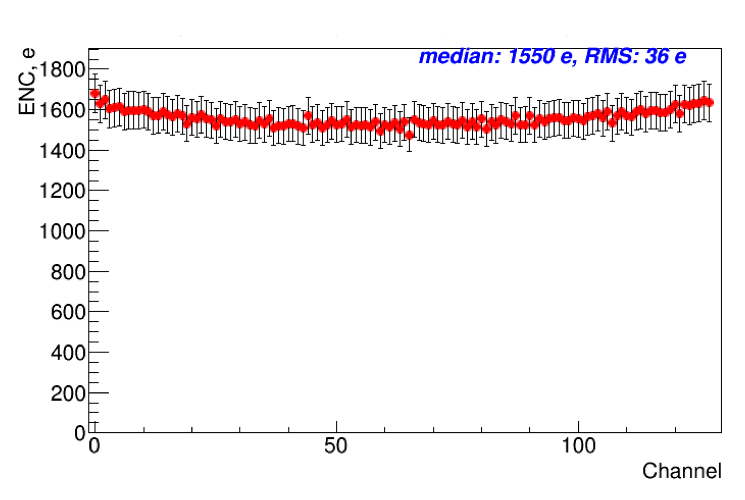
\includegraphics[width=0.8\columnwidth,keepaspectratio]{enc-chip.png}
\caption{Typical input noise on a single chip of an SVT module.}
\label{fig:enc-chip}
\end{figure} 

Detailed quality assurance procedures were developed for testing the modules during assembly at Fermilab, reception tests at Jefferson Lab, tracker integration, and commissioning. At each stage the results were compared with previous measurements. Module performance was tested by calibration procedures. No significant correlated noise has been observed between the channels of the same chip, chips of the same module or closely placed modules. The measured average channel noise (see Fig.~\ref{fig:enc-chip}) is comparable with the estimated contributions of different noise sources. The gain dispersion measured on the channels is within the specs of the readout chip (see Fig.~\ref{fig:gain-chip}).

\begin{figure}[hbt] 
\centering 
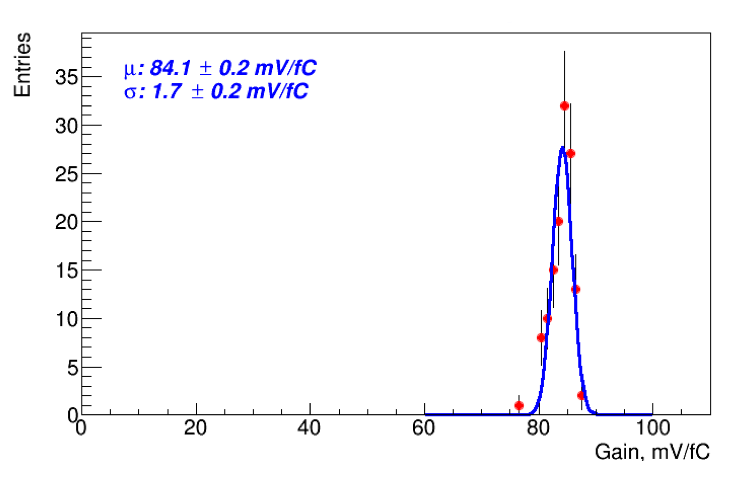
\includegraphics[width=0.8\columnwidth,keepaspectratio]{gain-chip.png}
\caption{Distribution of the gain for the channels of one representative FSSR2 ASIC.}
\label{fig:gain-chip}
\end{figure}

\begin{figure}[hbt] 
	\centering 
	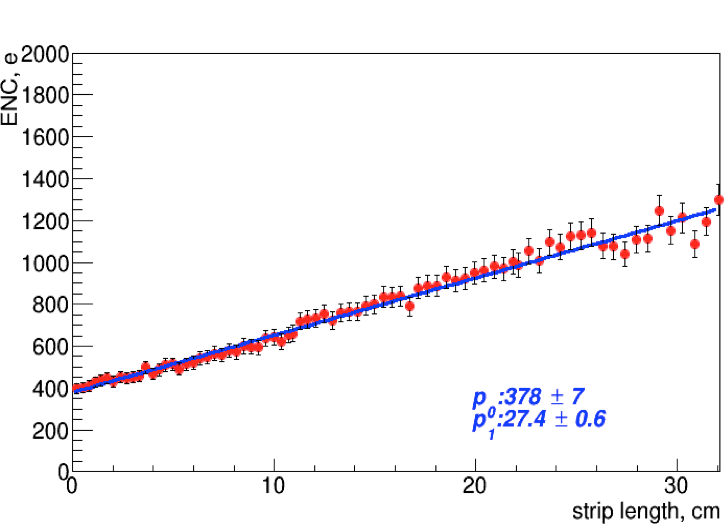
\includegraphics[width=0.8\columnwidth,keepaspectratio]{encstriplength.png}
	\caption{Input noise vs. strip length.}
	\label{fig:encstriplength}
\end{figure}

Longer silicon strips have higher capacitance and thus a higher input noise (see Fig.~\ref{fig:encstriplength}). Noise calibration accounts for the different strip lengths and pitch adapter layouts that affect the input capacitance of the preamplifier. The mean noise values scale linearly with strip length which confirms that the noise is dominated by the strip capacitance and not by coherent noise pickup of the system. The channel noise has a linear dependence on the strip length with the offset p$_{0}$ about 400 electrons corresponding to the ENC for the shortest strips and the slope p$_1$ of 27 electrons, consistent with expected FSSR2 noise performance at comparable capacitive load (see Fig.~\ref{fig:fssr2-enc-c}).

\begin{figure}[hbt] 
\centering 
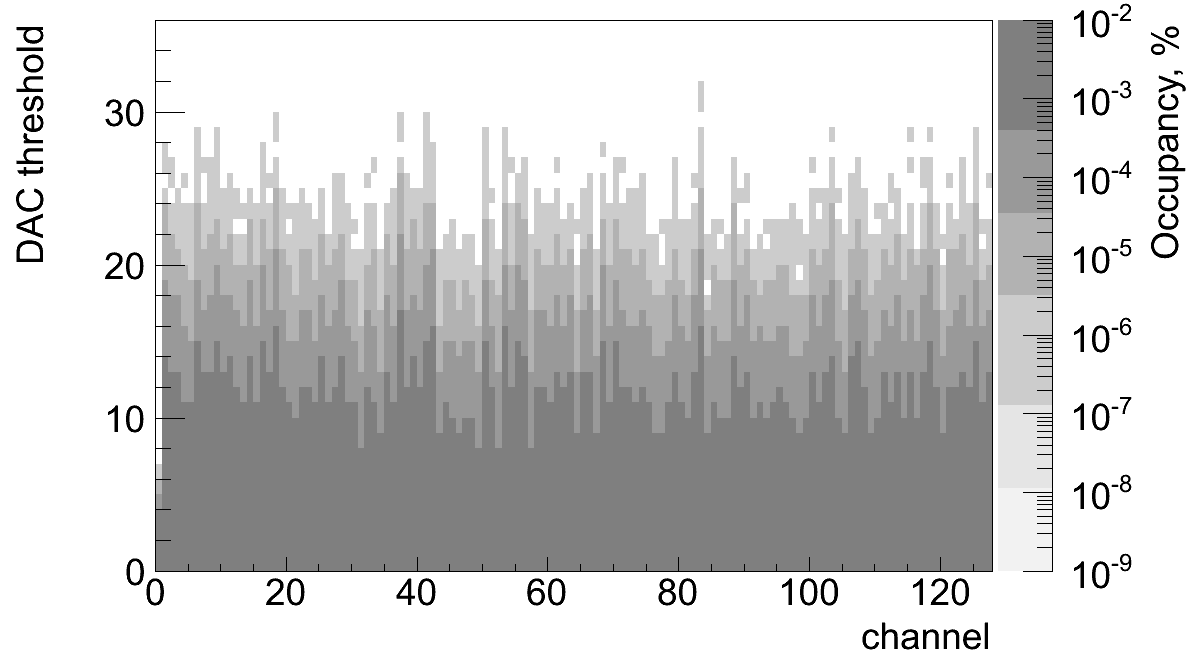
\includegraphics[width=1.0\columnwidth,keepaspectratio]{occ_thr.png}
\caption{Channel noise occupancy vs. DAC hit/no-hit threshold (in DAC bins, one DAC bin corresponds to 3.5~mV).}
\label{fig:noiseocc}
\end{figure}

The noise occupancy histogram with no charge injection is shown in Fig.~\ref{fig:noiseocc}. It probes the tail of the noise distribution, which can show effects masked by the higher occupancy at low thresholds. Channel noise allows setting a 3~$\sigma$ threshold at the 30~keV level. The Equivalent Noise Charge (ENC) of the SVT channels is shown in  Fig.~\ref{fig:enc}. The peak is $\sim$1600 electrons, the shoulder on the left side corresponds to the shorter strips. The channel noise allows setting a 3$\sigma$ threshold at the 20~keV level. 

\begin{figure}[hbt] 
	\centering 
	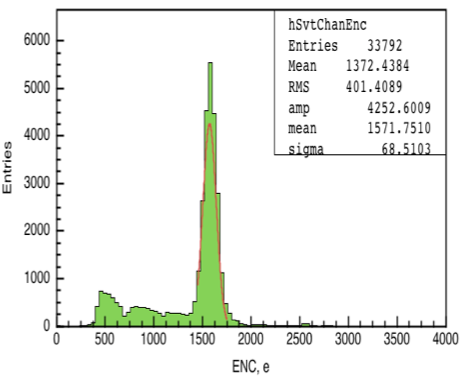
\includegraphics[width=1.0\columnwidth,keepaspectratio]{enc.png}
	\caption{SVT noise for all channels. The main peak corresponds to the full length strips (33 cm). The shoulder on the left side corresponds to the shorter strips.}
	\label{fig:enc}
\end{figure}

The detector response and full readout chain calibration was done with $\gamma$ and $\beta$ sources, cosmic muons, electron beam, and proton beam. The output from the 3-bit ADC is not allowing to get a good resolution of the pulse height. To increase the number of bins in the cluster charge distribution, a sliding window method was used, combining the data taken for the same time window in several runs with discriminator thresholds set for the required binning. When using signals from minimum ionizing particles, like cosmic rays or $^{90}$Sr $\beta$ source, the signal distribution is fitted with a Landau-Gauss convolute. The detector response to minimum ionizing particles was about 24000 electrons, which is what is expected for the 320 $\mu$m thick sensor. The results of absolute gain calibration with a $\gamma$ source are shown in Fig.~\ref{fig:signal-gamma}. The signal peak is in good agreement with the expected position. 

\begin{figure}[hbt] 
	\centering 
	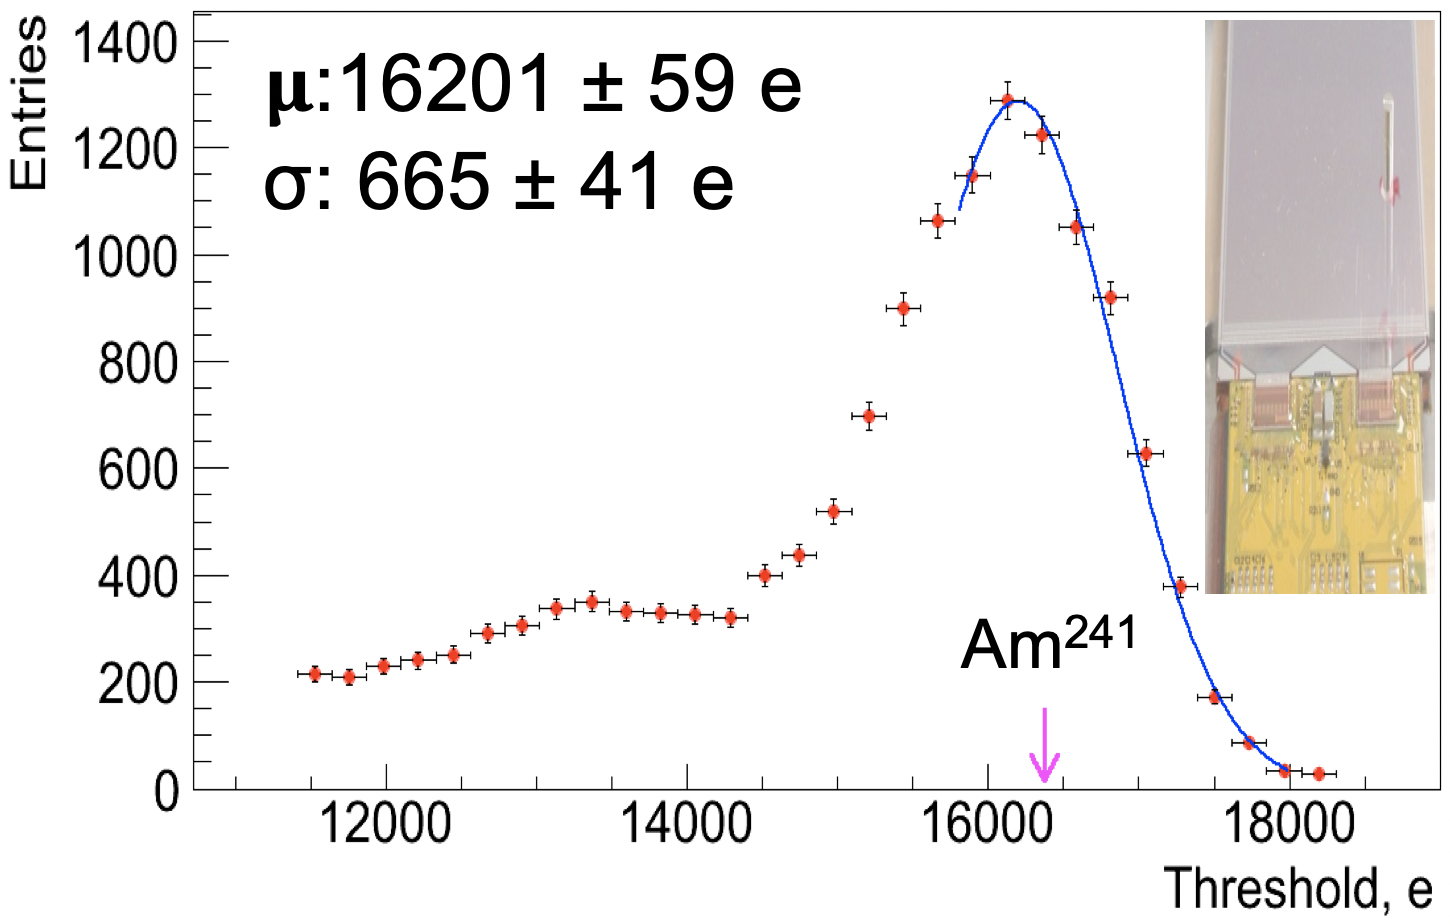
\includegraphics[width=0.8\columnwidth,keepaspectratio]{signal-gamma.png}
	\caption{Signal from Am$^{241}$ $\gamma$ source.}
	\label{fig:signal-gamma}
\end{figure}

%
%\begin{wrapfigure}{l}{0.5\columnwidth}
%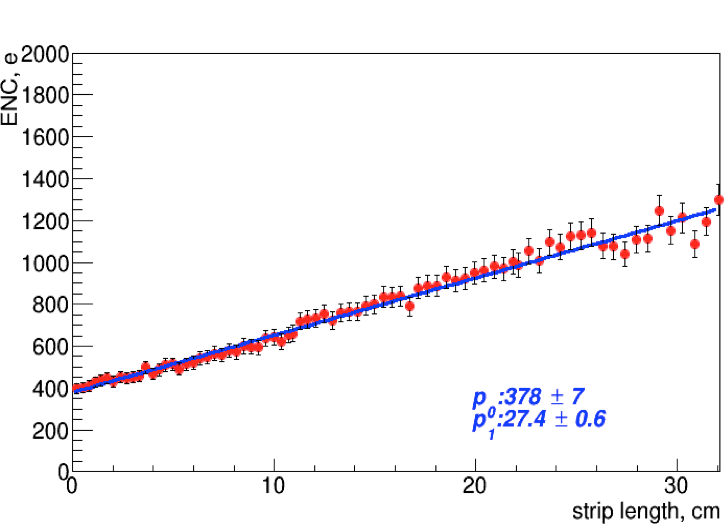
\includegraphics[width=1.0\columnwidth]{encstriplength.png}
%\caption{Input noise vs. strip length.}
%\label{fig:encstriplength}
%\end{wrapfigure}
%Longer silicon strips have higher capacitance and thus a higher expected value for the input noise. 
%(see Fig.~\ref{fig:encstriplength}).
%

%\begin{wrapfigure}{l}{0.5\columnwidth}
%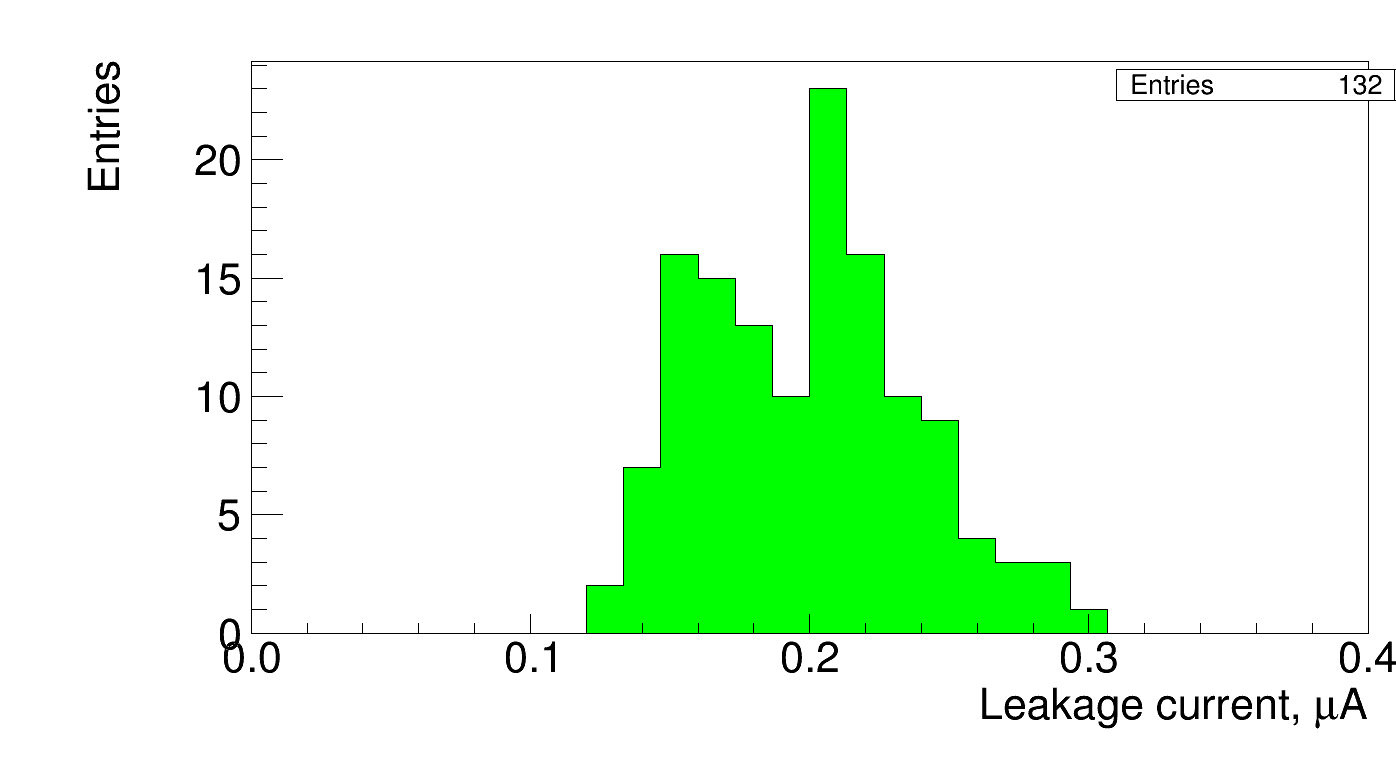
\includegraphics[width=1.0\columnwidth]{currents.png}
%\caption{Leakage currents}
%\label{fig:currents}
%\end{wrapfigure}
%
%\begin{wrapfigure}{l}{0.5\columnwidth}
%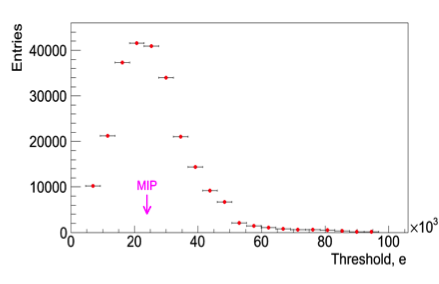
\includegraphics[width=1.0\columnwidth]{signal-muons.png}
%\caption{Signal muons}
%\label{fig:signal-muons}
%\end{wrapfigure}

\subsection{Integration and system checkout}

To verify performance of the integrated detector, data acquisition chain, power services, and cooling system, as well as the detector control and data acquisition software, the final detector system was installed in the clean room and used at all stages of tracker integration and commissioning. The SVT was operated for several months under environmental conditions close to the ones in the experimental hall. Defects known before the integration of the system were reestablished. 99.9$\%$ of channels were operational after the detector integration. 

\begin{figure}[hbt] 
\centering 
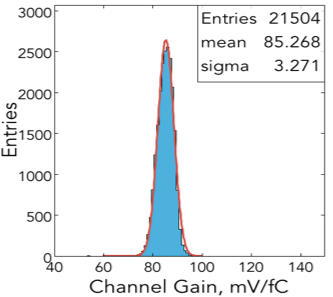
\includegraphics[width=0.8\columnwidth,keepaspectratio]{svt_gain.png}
\caption{Distribution of gain for the SVT channels.}
\label{fig:svt_gain}
\end{figure}

The noise behavior was found to be within expectations and well understood. The dependence of the noise on the environmental temperature and humidity is small. The noise performance in the experimental hall was comparable with the results taken in the clean room during integration. No significant correlated noise has been observed between the channels of the same chip, between the chips of the same module, or between the closely placed modules. The front-end electronics performed reliably, and no chip failures were observed. 
 
\begin{figure}[hbt] 
\centering 
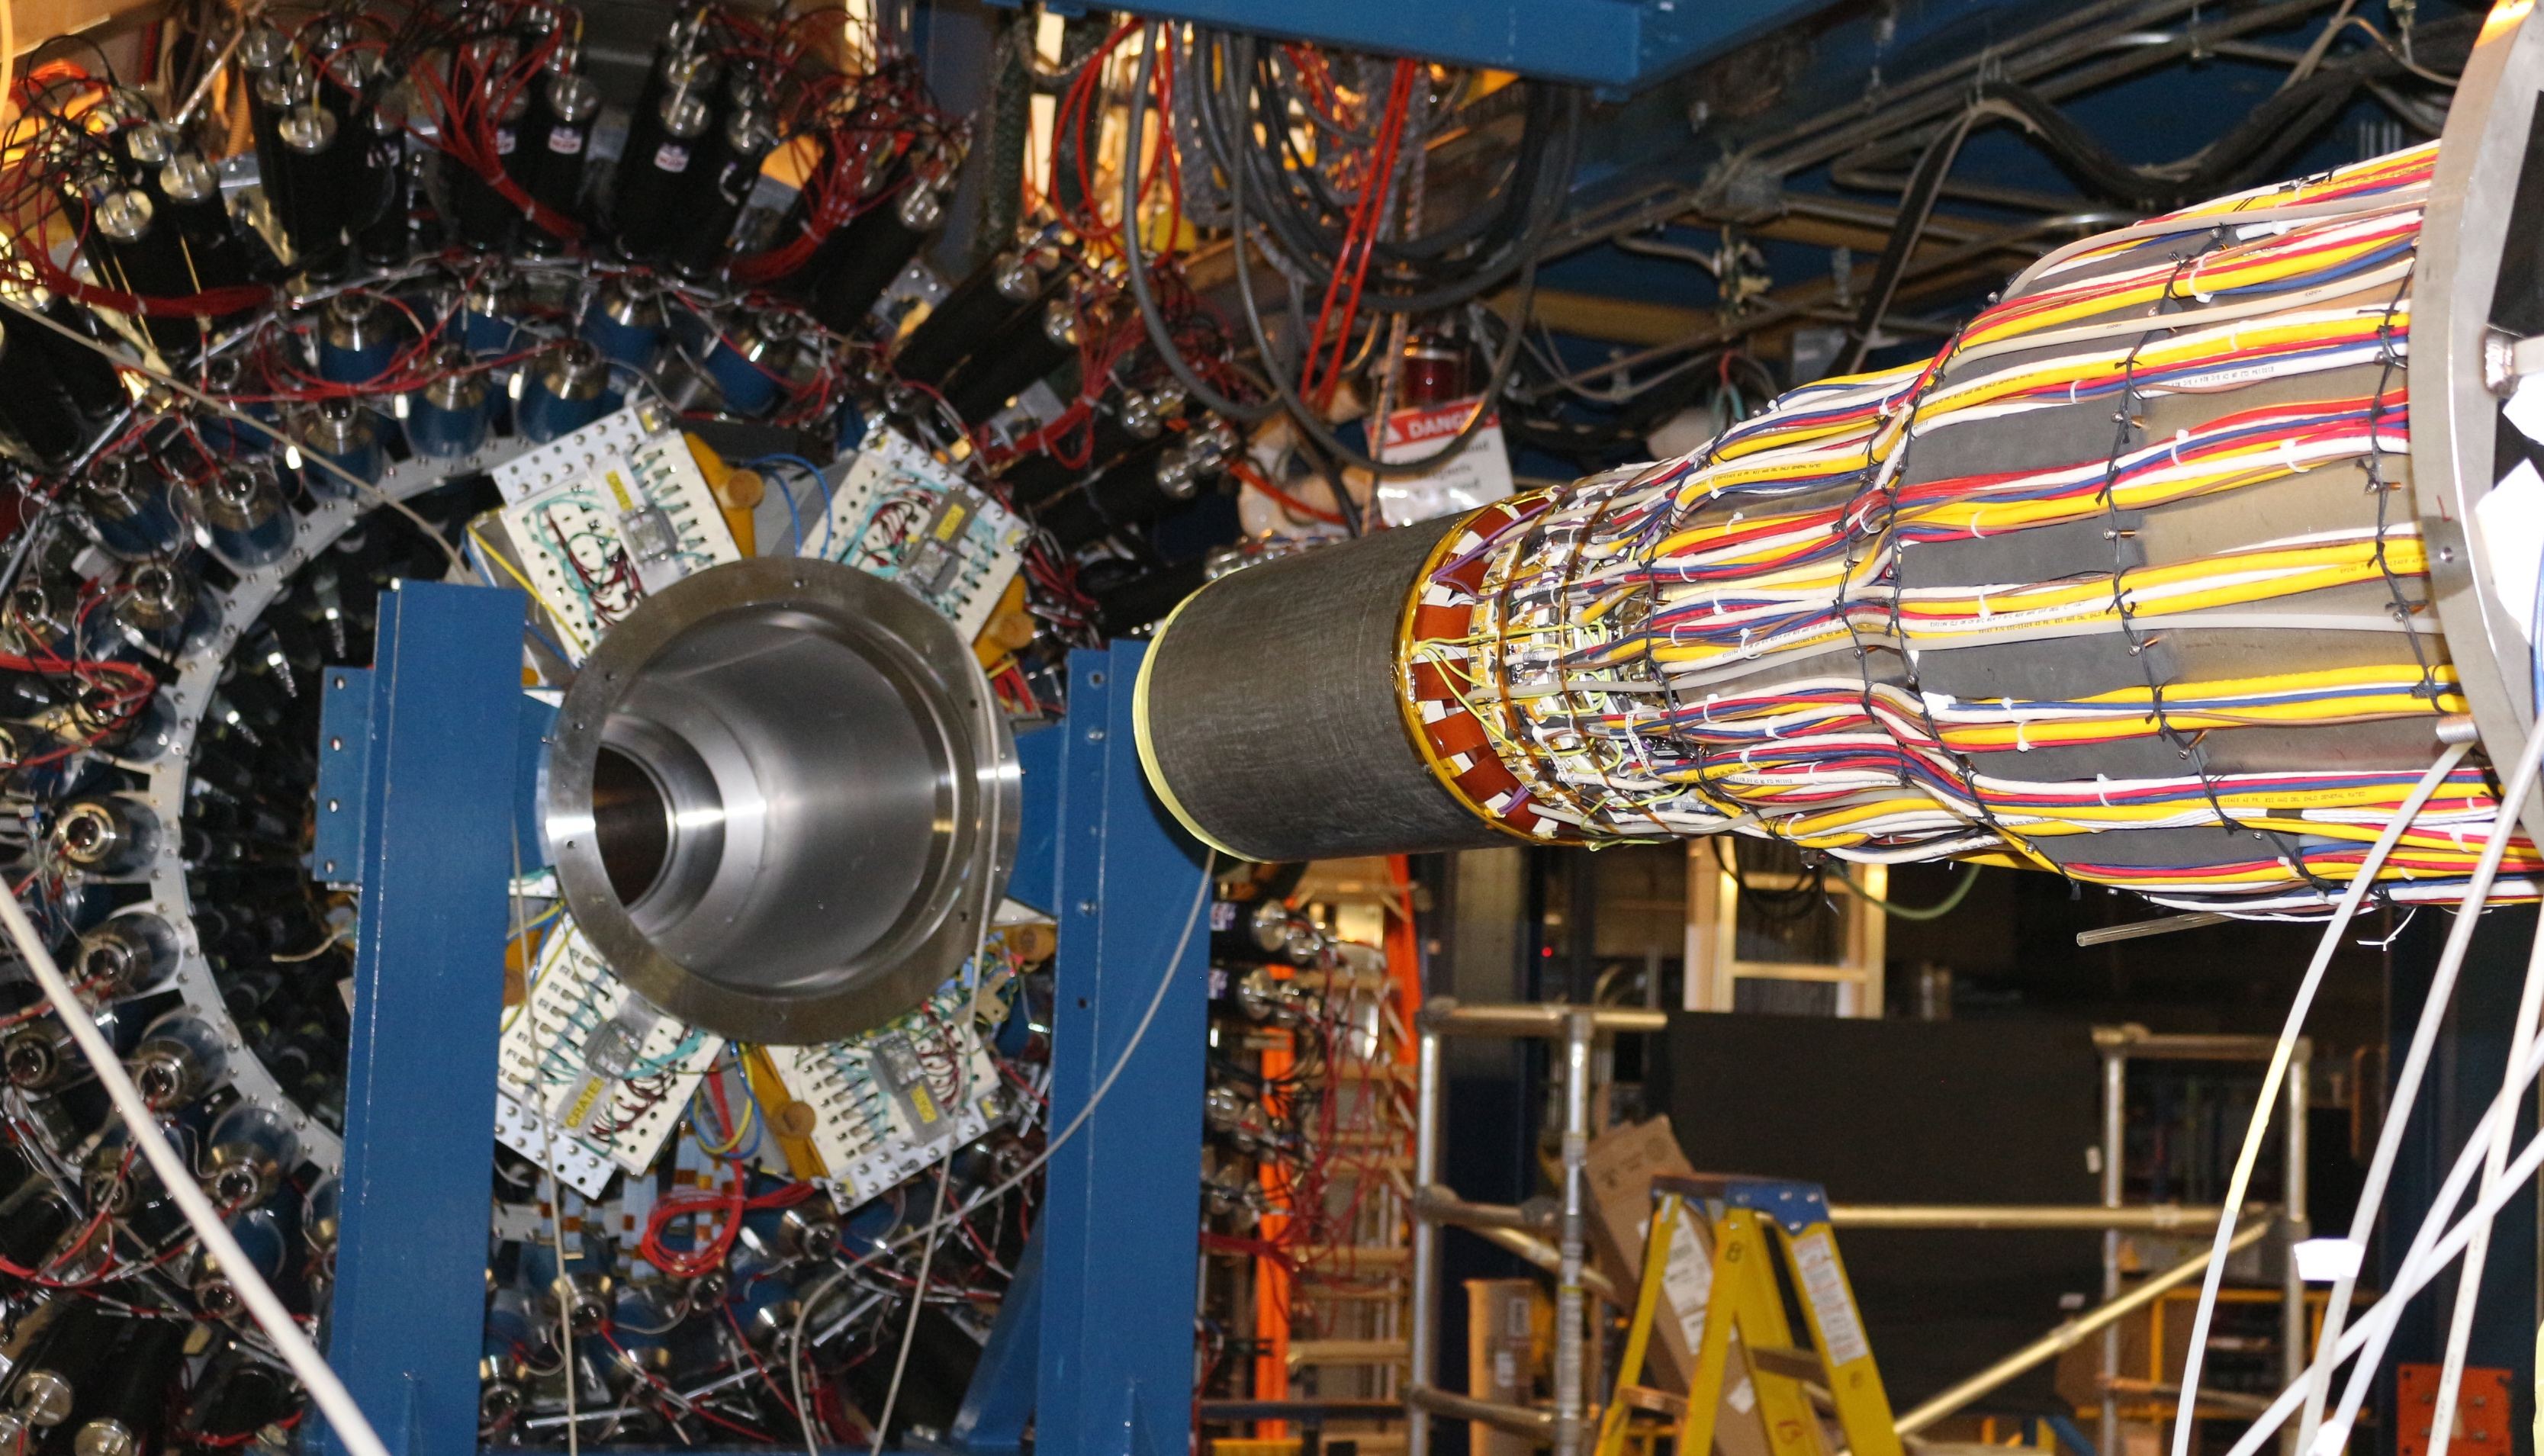
\includegraphics[width=1.0\columnwidth,keepaspectratio]{svt-hall.png}
\caption{SVT detector installed in the experimental hall before being pushed inside the CLAS12 detector.}
\label{fig:svt-hall}
\end{figure}

The distribution of gain was uniform and stable for all channels (see Fig.~\ref{fig:svt_gain}). All modules were found to be fully functional after transportation from the assembly site and installation on the beam line. Fig.~\ref{fig:svt-hall} shows the SVT detector after installation in the experimental hall.

\begin{figure}[hbt] 
\centering 
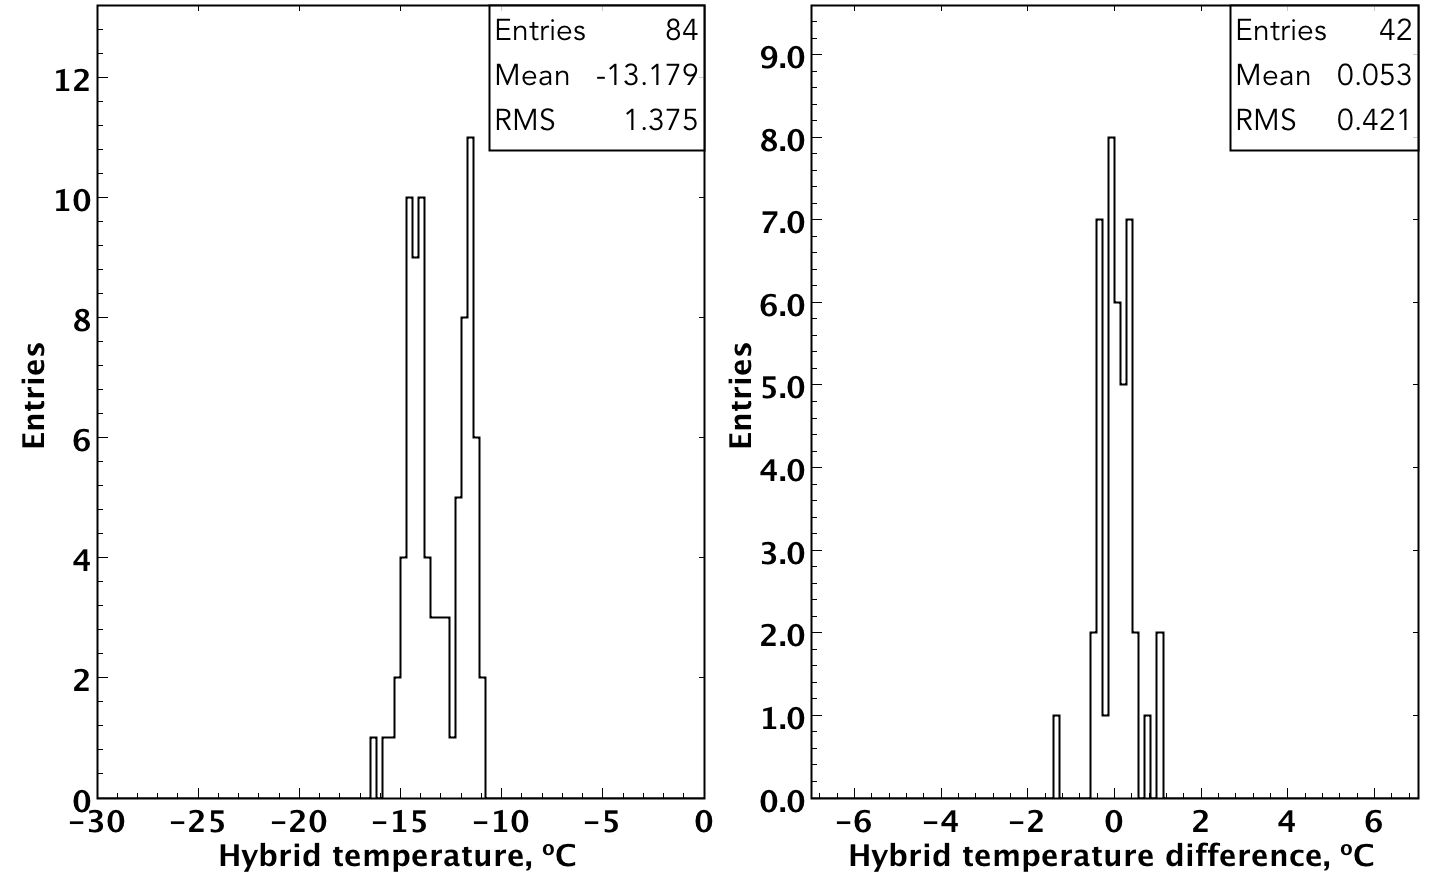
\includegraphics[width=1.0\columnwidth,keepaspectratio]{hybrid-temps.png}
\caption{Hybrid temperatures (left) and the difference in temperature between the two sides of the module with coolant at -26 $^\circ$C (right).}
\label{fig:hybrid-temps}
\end{figure}

Temperature variation of the SVT modules measured by sensors mounted on the hybrids with coolant at -26 $^\circ$C is shown in Fig.~\ref{fig:hybrid-temps} (left). In these operating conditions the module temperatures were uniformly distributed within the region, with lower temperatures close to the cooling lines. Region 3 temperatures were slightly higher than in the inner regions. The temperature difference between the two sides of a module is within 1$^\circ$C as shown in Fig.~\ref{fig:hybrid-temps} (right). Sensor leakage currents remained at the same low levels after installation (see Fig.~\ref{fig:currents}). Thermal cycling of the modules verified the robustness of the bond wires.

\begin{figure}[hbt] 
\centering 
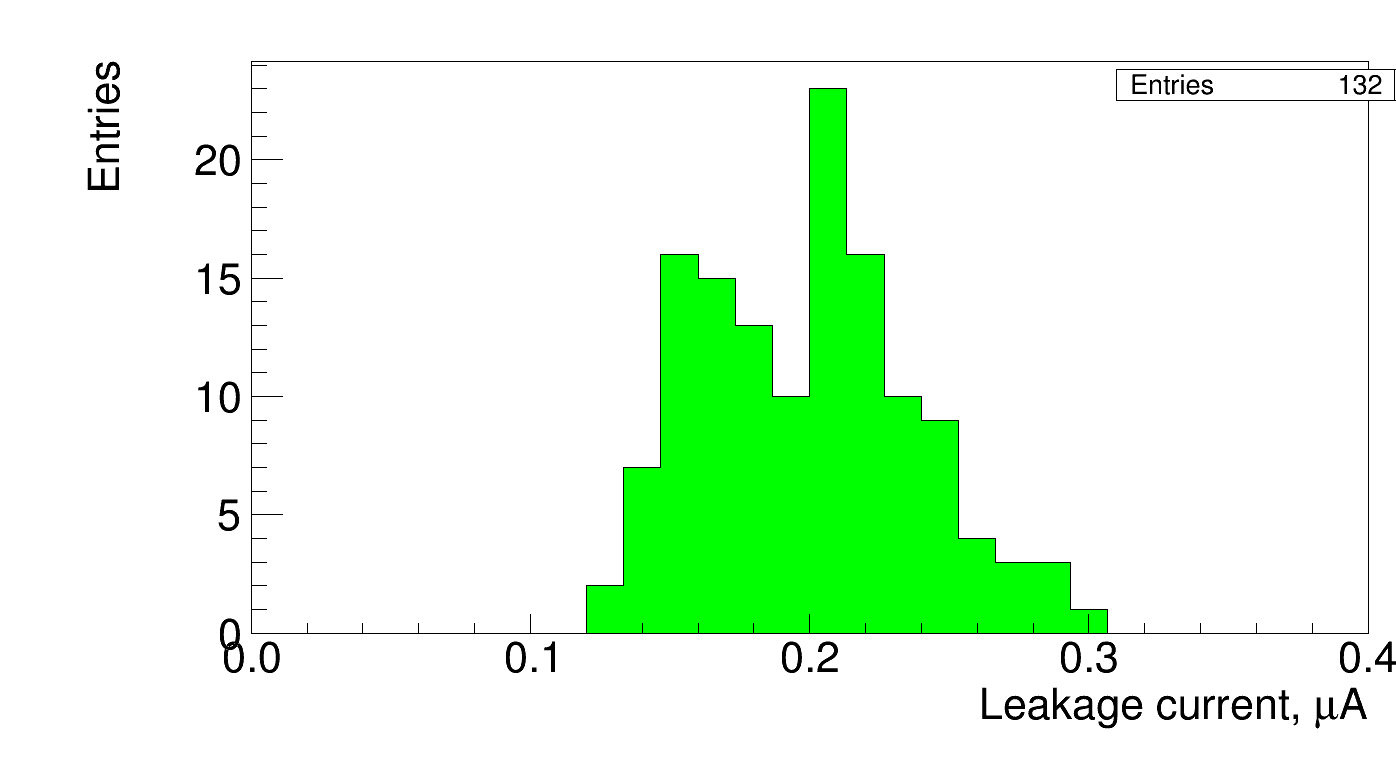
\includegraphics[width=1.0\columnwidth,keepaspectratio]{currents.png}
\caption{Sensor leakage currents after detector integration.}
\label{fig:currents}
\end{figure}

\subsection{Commissioning with cosmic rays}

Cosmic ray tests of the SVT have been used to test track reconstruction routines for the SVT, as well as to establish correct readout, good noise performance, and full response for the entire detector. Cosmic data during detector integration in the clean room were taken in the standalone mode using the self triggering feature of the FSSR2 readout chip in coincidence logic. VSCM boards reading the SVT modules located at the top and bottom halves of the horizontally placed barrel provided the trigger signals via signal distribution of two VXS crates. The coincidence of  signals from the trigger interface boards of both crates was taken as the cosmic trigger. The response of the channels was uniform, and performance results obtained during tracker integration were confirmed. The angular distribution of the cosmic muons reconstructed in the SVT is shown in Fig.~\ref{fig:track-phi-theta}.

\begin{figure}[hbt] 
\centering 
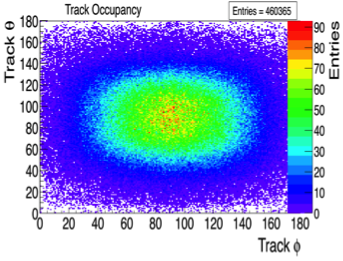
\includegraphics[width=0.9\columnwidth,keepaspectratio]{track-phi-theta.png}
\caption{Angular distribution of the cosmic muons reconstructed in the SVT.}
\label{fig:track-phi-theta}
\end{figure}

After installation of the SVT in the hall, a trigger from CTOF detector was used to collect cosmic data for the CLAS12 central detector. A cosmic muon reconstructed in the central detector is shown in Fig.~\ref{fig:cd-cosmic-event}. SVT is the inner detector, surrounded by the BMT, the CTOF, and the CND. Yellow circles represent crosses in the SVT and green circles correspond to the clusters in the Micromegas detector. Between the physics data taking runs more cosmic trigger data were collected for calibration and performance studies.  A hit map for the SVT channels during the cosmic run is shown in Fig.~\ref{fig:cosmic-hitmap-svt}. Lower hit occupancy on the right side of the map is due to the shorter strips at this side of the sensors. After a year of running several sensors developed pinholes, observed as groups of adjacent hot channels. The bias voltage on these sensors has been lowered to reduce noise and abnormally high leakage currents (high occupancy regions on the map). The increased leakage current is reduced by lowering the detector temperature which is kept below -10 C to avoid reverse annealing.

\begin{figure}[hbt] 
\centering 
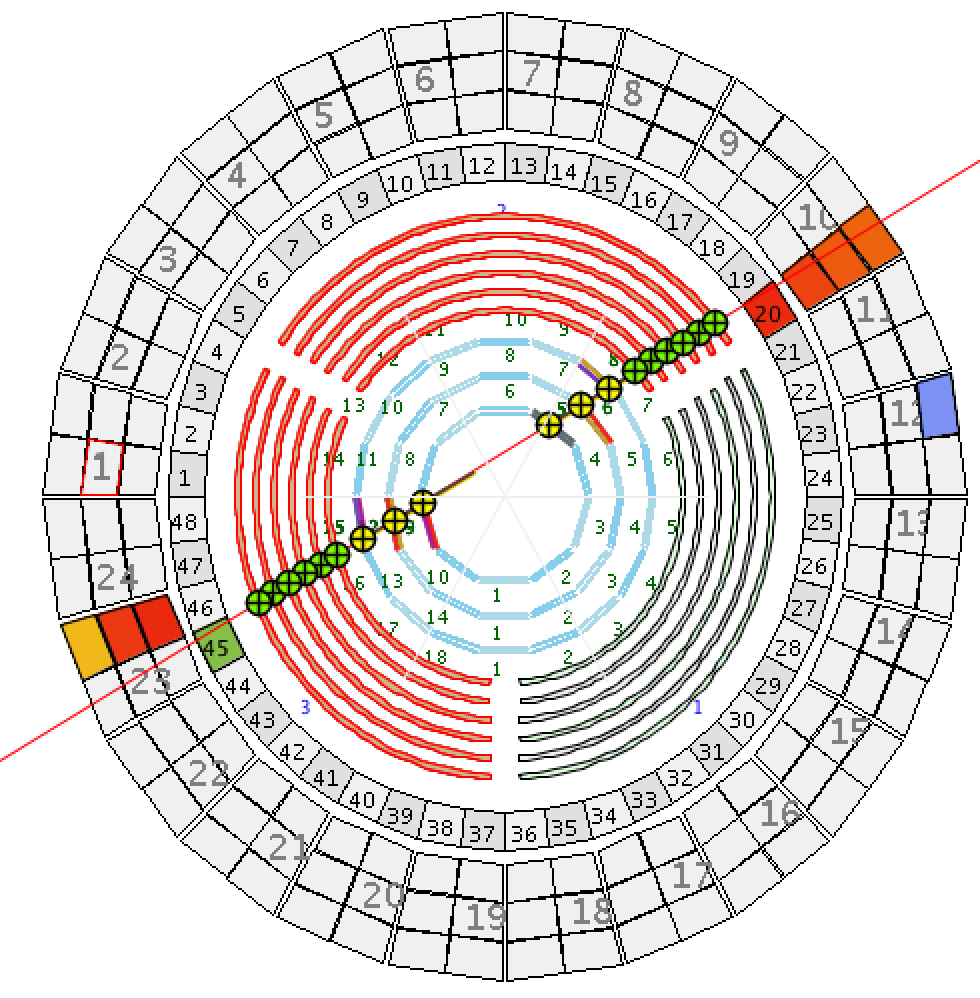
\includegraphics[width=0.6\columnwidth,keepaspectratio]{cd-cosmic-event.png}
\caption{Cosmic muon reconstructed in the CLAS central detector.}
\label{fig:cd-cosmic-event}
\end{figure}

\begin{figure}[hbt] 
\centering 
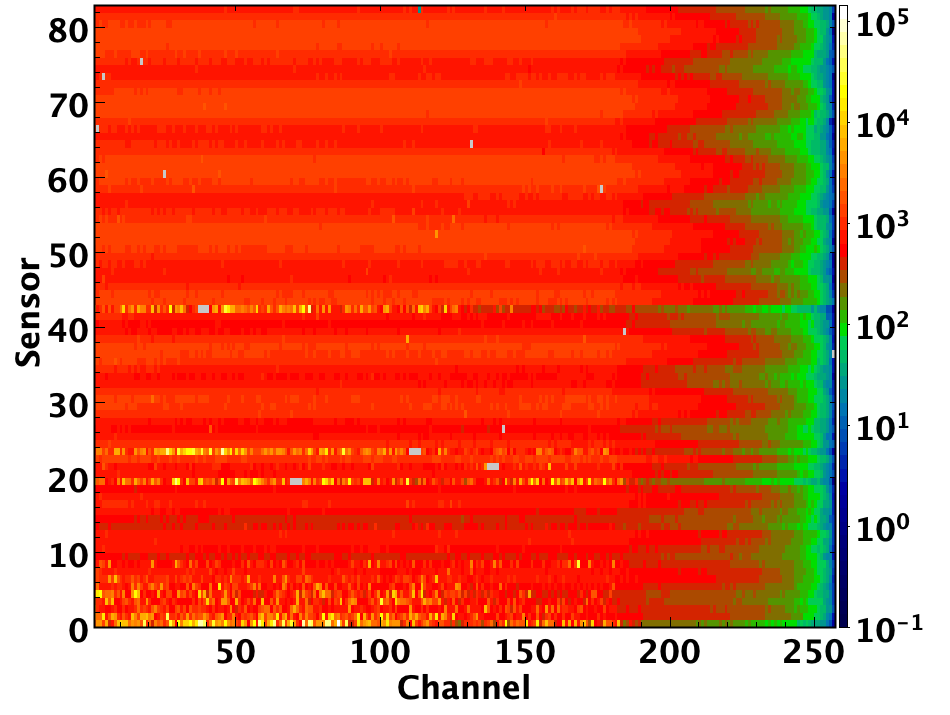
\includegraphics[width=0.9\columnwidth,keepaspectratio]{cosmic-hitmap-svt.png}
\caption{Monitoring SVT hit map during a cosmic run showing module vs. strip number.}
\label{fig:cosmic-hitmap-svt}
\end{figure}

The charge sharing among two adjacent strips was studied using using the $\eta$-function, defined for the 2-strip clusters as the ratio of the pulse height of the left strip to the pulse height of the cluster. Fig.~\ref{fig:eta-function} shows the  $\eta$-function obtained from the measurement of on-track clusters from the cosmic muons. The granularity of the pulse height after the digitization is coarse due to the 3-bit ADC of the readout chip. There is a pronounced peak in the center between the two readout strips where all the charge is collected by the intermediate strip. Because of capacitive coupling, signals on these intermediate strips are partially transferred to the readout strips.

\begin{figure}[hbt] 
\centering 
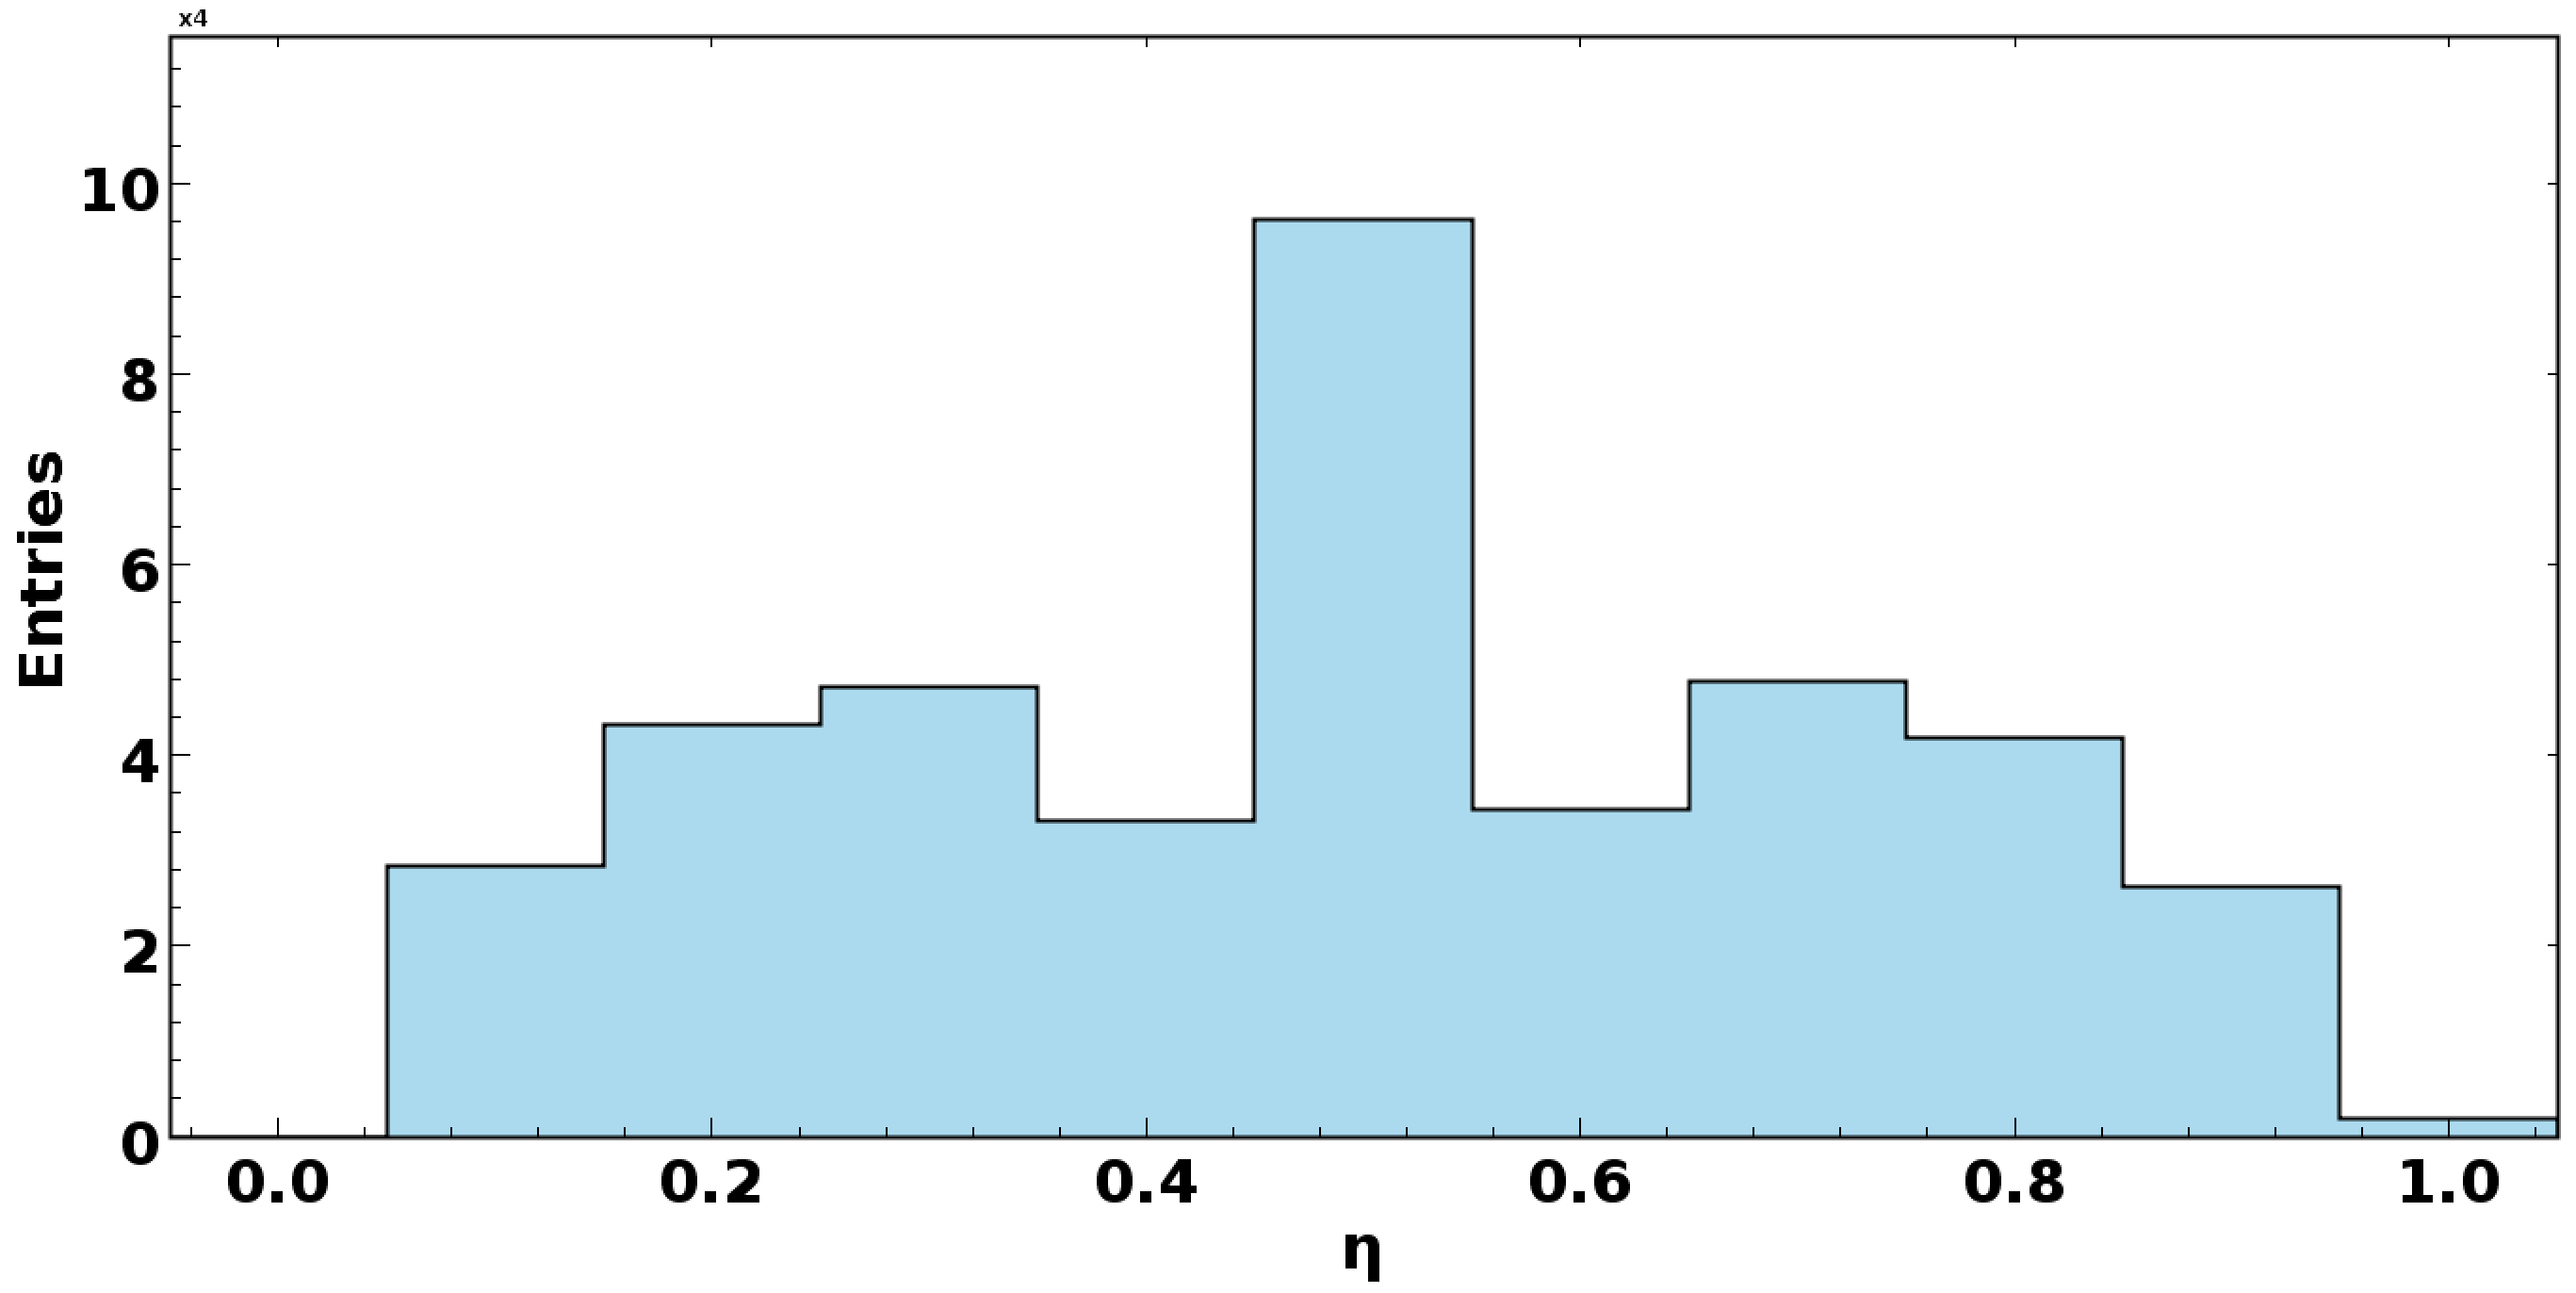
\includegraphics[width=0.8\columnwidth,keepaspectratio]{eta-function.png}
\caption{$\eta$-function for the two-strip clusters.}
\label{fig:eta-function}
\end{figure}

Strip multiplicity of the clusters (cluster size) in the cosmic run is shown in Fig.~\ref{fig:cluster-size}. The size of the clusters is lowest in the innermost region and is increasing with radius due to a larger local track angle (the tracks, triggered by the CTOF, crossing the barrel far from the beam line).

\begin{figure}[hbt] 
\centering 
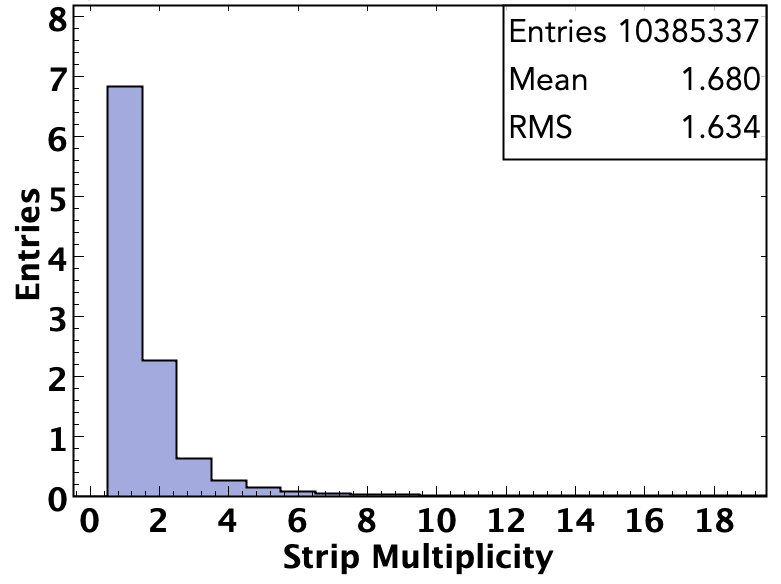
\includegraphics[width=0.8\columnwidth,keepaspectratio]{cluster-size.png}
\caption{Strip multiplicity of the clusters in the cosmic run.}
\label{fig:cluster-size}
\end{figure}

Cosmic muons are an important source for calibration and alignment. Their trajectories are sensitive to misalignments of different tracker parts. The cosmic muons significantly improve the alignment precision. A preliminary alignment of the SVT was done using the sample of several millions of the cosmic muon tracks taken without solenoid magnetic field. With exception of the modules located at the shallow angle to the vertical axis, the acquired sample provided adequate statistics of the tracks to extract the misalignment data. The tracks crossing the sensors at large inclination angles and low energy tracks subject to multiple scattering were rejected. Additional requirement on the $\chi^2$ per degree of freedom of the track fit was applied to reject tracks effected by the outlier hits. The spacial residuals before (blue) and after (red) the alignment procedure (see Fig.~\ref{fig:alignment}) are expected to provide the designed momentum resolution.

\begin{figure}[hbt] 
\centering 
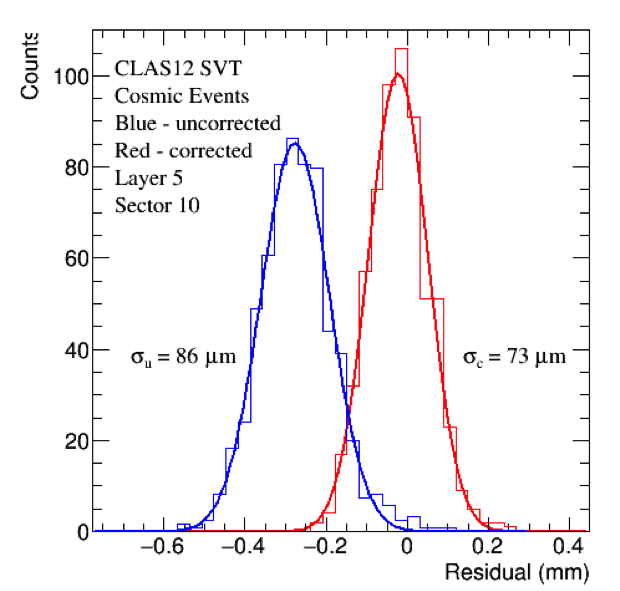
\includegraphics[width=0.8\columnwidth,keepaspectratio]{alignment.png}
\caption{Residuals for one of the SVT sensors before (blue) and after (red) alignment.}
\label{fig:alignment}
\end{figure}

\subsection{Commissioning with beam}
The front-end electronics performance and noise occupancy of the detector were studied during physics data taking. No interference with other CLAS12 subsystems were found. The data quality and detector operational stability  were verified with both online and offline monitoring packages. There were occasional FSSR2 chip latch-ups observed after the start of a new run. These latch-ups were traced by improper configuration of the chips and fixed by adding additional resets to the run start sequence.

\begin{figure}[h] 
\centering 
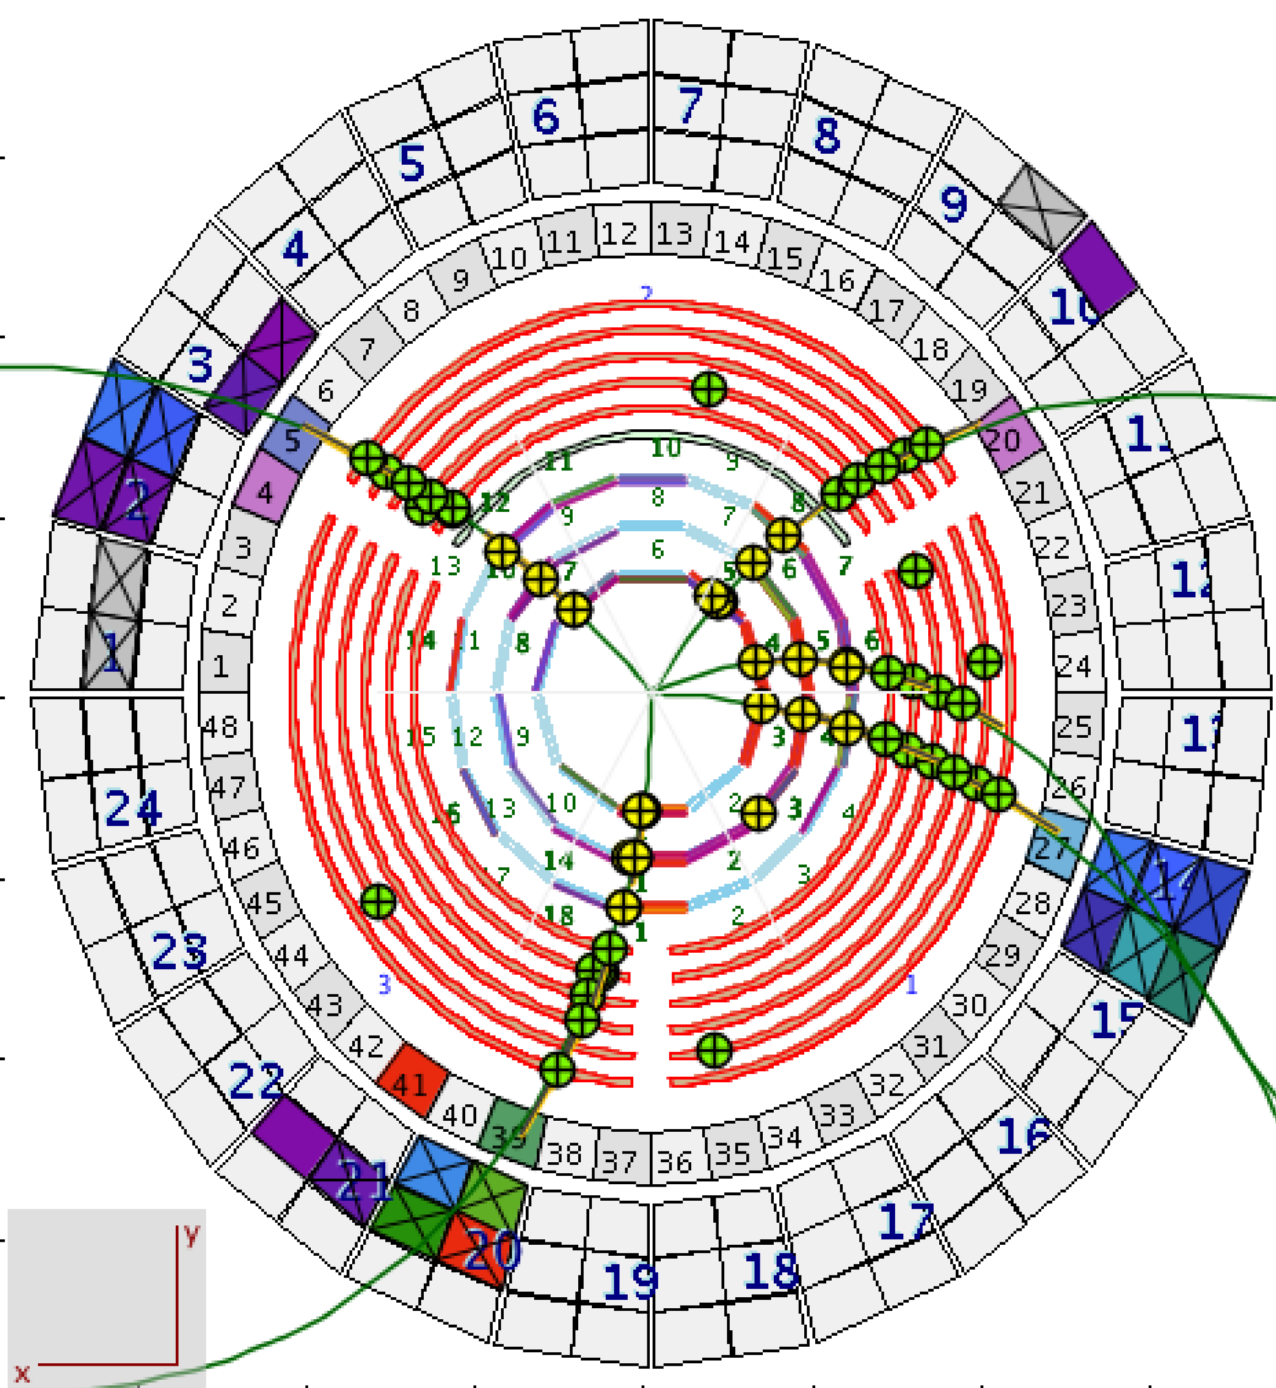
\includegraphics[width=0.6\columnwidth,keepaspectratio]{cd-tracks.png}
\caption{Multi-track event reconstructed in the CLAS12 central detector during a physics run.}
\label{fig:cd-tracks}
\end{figure}

Tracks reconstructed in the CLAS12 central detector during a physics run are shown in Fig.~\ref{fig:cd-tracks}. The level-1 trigger latency is finely tuned to match the CLAS12 trigger delays.

\begin{figure}[htb] 
\centering 
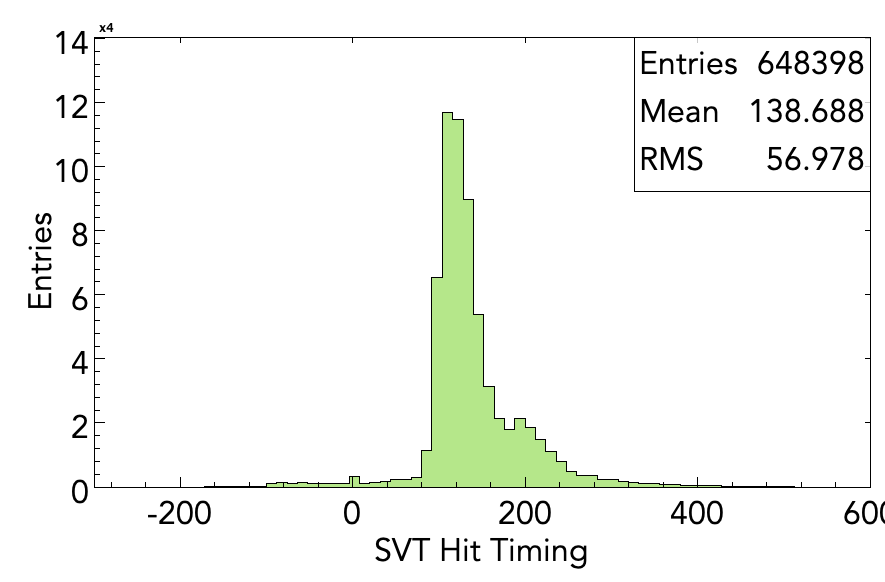
\includegraphics[width=0.9\columnwidth,keepaspectratio]{svt-hit-timing.png}
\caption{SVT hit timing referenced to the CTOF time in a physics run with the hydrogen target.}
\label{fig:svt-hit-timing}
\end{figure}

FSSR2 readout chip does not provide the timing information from the hit. Reading the time stamp associated with a hit was implemented in the VSCM board. The time stamp is synchronized with the "Got Hit" pulse from the chip when the pulse height reaches the threshold set for the first discriminator of the ADC. Timing of the SVT hits referenced to the CTOF timing are shown in Fig.~\ref{fig:svt-hit-timing}. The data correspond to the time difference between the SVT and the CTOF time stamps for the SVT hits which were associated with a track. Applying a cut on this difference can be  used to remove background and noise hits in the track seeding algorithm.

\begin{figure}[hbt] 
\centering 
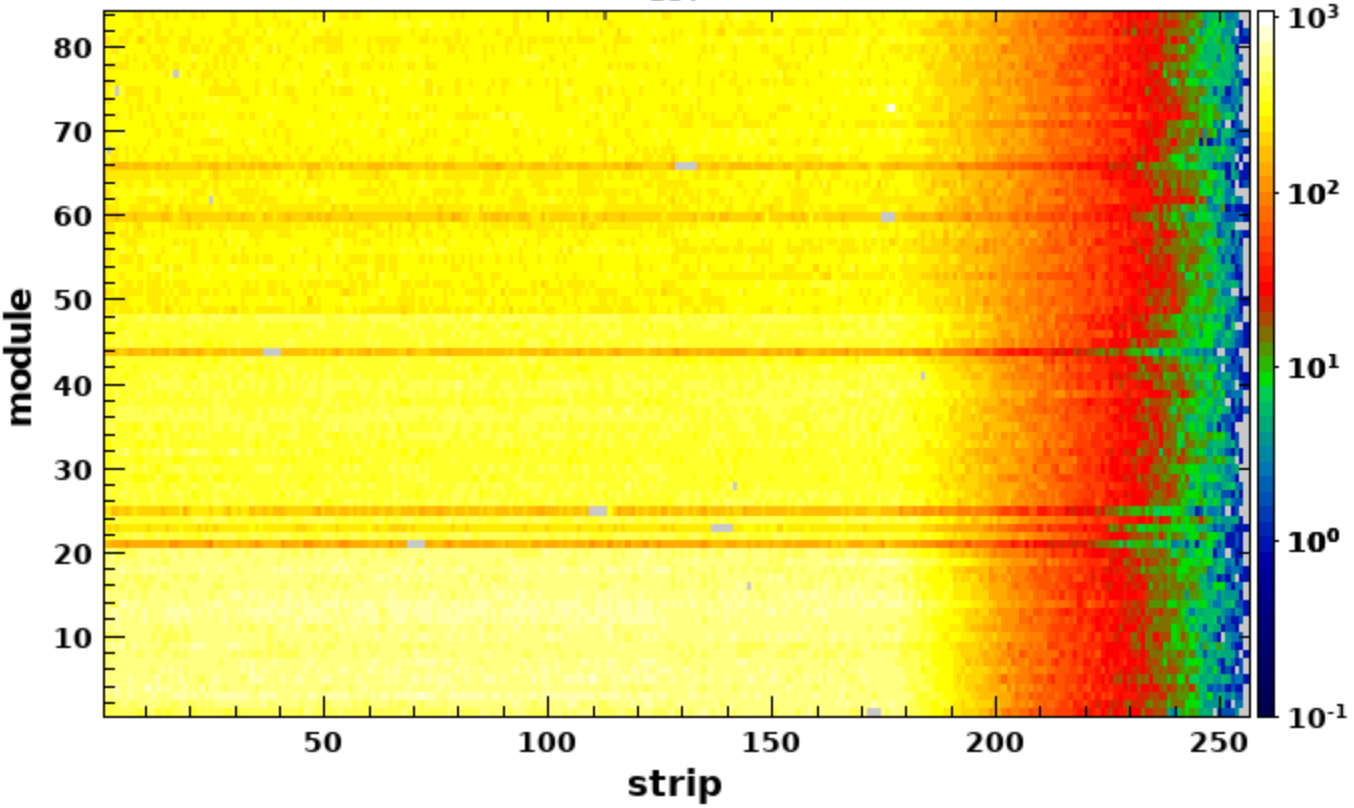
\includegraphics[width=0.9\columnwidth,keepaspectratio]{hit-map-rga.png}
\caption{SVT hit map during a physics run with the hydrogen target.}
\label{fig:hit-map-rga}
\end{figure}

A hit map of the SVT from a physics run is shown in Fig.~\ref{fig:hit-map-rga}. Sensors with pinholes are seen on the map as darker horizontal lines due to reduced efficiency (under-depleted sensors) with strips of masked hot channels. 

\begin{figure}[hbt] 
\centering 
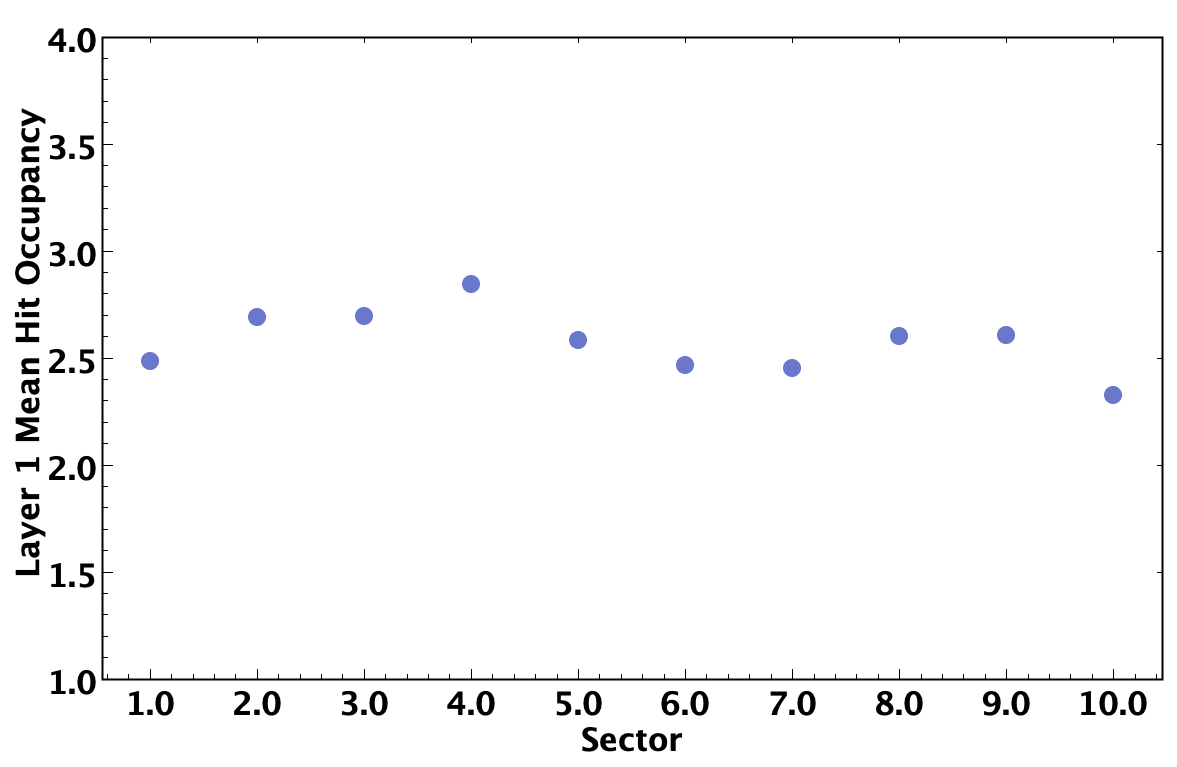
\includegraphics[width=1.0\columnwidth,keepaspectratio]{mean-hit-occupancy.png}
\caption{Mean hit occupancies for the sectors of the innermost SVT layer with hydrogen target at 50 nA beam current.}
\label{fig:mean-hit-occupancy}
\end{figure}

Fig.~\ref{fig:mean-hit-occupancy} shows average hit occupancy per event in the innermost SVT layer for the data taken with hydrogen target at nominal beam current of 50 nA. The hits are uniformly distributed among the sectors with occupancies close to 1$\%$ (each sensor has 256 strips).

\begin{figure}[hbt] 
\centering 
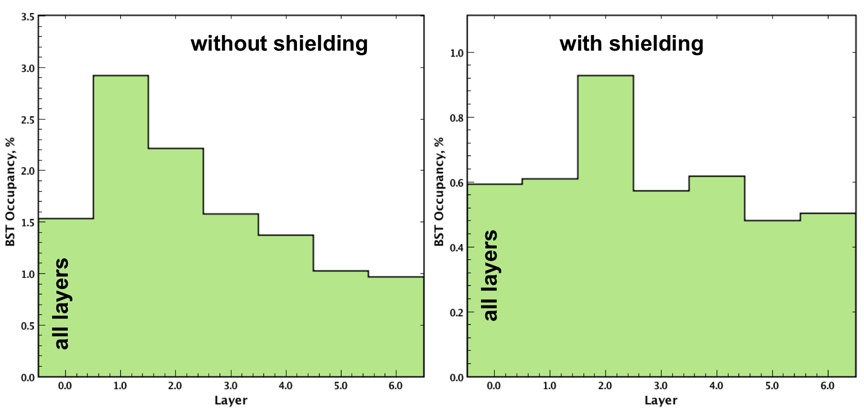
\includegraphics[width=1.0\columnwidth,keepaspectratio]{hit-occupancy-shielding.png}
\caption{Hit occupancies with and without the 50~$\mu$m-thick tungsten shield installed outside of the target scattering chamber.}
\label{fig:hit-occupancy-shielding}
\end{figure}

The impact of the tungsten shield on the SVT occupancy is shown in Fig.~\ref{fig:hit-occupancy-shielding}. Occupancies in all SVT layers are substantially lower, which results in better tracking performance due to reduced combinatorics. The effect of the shield on momentum resolution is negligible~\cite{SHIELDNOTE}. For the liquid hydrogen target the occupancy in the innermost layer of the SVT is approximately 1$\%$, decreasing to 0.5$\%$ in the outermost layer. There is no hit efficiency loss due to the dead time of the readout system at such occupancies.
